% Diplomový projekt 2017/2019
% Matúš Cuper

%-------------------------------------------------------------------------------
%   PACKAGES AND DOCUMENT CONFIGURATION
%-------------------------------------------------------------------------------

\documentclass[a4paper,twoside,slovak,12pt]{article}

\usepackage[slovak]{babel}                                                      % title in Slovak
\usepackage[IL2]{fontenc}                                                       % support for word wrapping of special Slovak characters at the end of line on the end
\usepackage[utf8]{inputenc}                                                     % support for special Slovak characters
\usepackage{enumitem}																														% support for itemize
\usepackage{times}																															% Times New Roman
\usepackage[unicode]{hyperref}																									% hyperreferences in table of content
\usepackage{amsmath}                                                            % math fractions
\usepackage{amssymb}                                                            % real numbers sign
\usepackage{algorithm, algpseudocode}                                           % pseudocode writting
\usepackage{graphicx}                                                           % figures
\usepackage{threeparttable}                                                     % table with footnotes
\usepackage{url}                                                                % url in references
\usepackage{listings}                                                           % source code syntax highlighting
\usepackage{courier}																														% monospace in listings
\usepackage{caption}																														% enable caption centering
\usepackage[a4paper, centering,
											left=35mm, top=25mm, right=20mm, bottom=25mm]{geometry}		% set page margins

\lstset{
    basicstyle=\ttfamily,
		breaklines=true,
    postbreak=\raisebox{0ex}[0ex][0ex]{\ensuremath{\color{red}\hookrightarrow\space}}
}

\graphicspath{ {img/} }		                                                      % set path for figures

\hypersetup{																																		% with default colours for links
    colorlinks,
		pageanchor=false,
    citecolor=black,
    filecolor=black,
    linkcolor=black,
    urlcolor=black
}

%-------------------------------------------------------------------------------
%   TITLE PAGES
%-------------------------------------------------------------------------------

\begin{document}
\begin{titlepage}
	\centering
	{\Large Slovenská technická univerzita v Bratislave \par}
	{\Large Fakulta informatiky a informačných technológií \par}
  \vspace{0.5cm}
  {\normalsize Evidenčné číslo: FIIT-0000-73688 \par}
	\vspace{7cm}
  {\large Bc. Matúš Cuper \par}
  \vspace{0.5cm}
	{\LARGE Identifikácia neštandardného správania odberateľov v energetickej sieti \par}
	\vspace{0.5cm}
	{\large Diplomová práca \par}
	\vspace{7cm}
  \flushleft
	{\large Vedúci práce: Ing. Marek Lóderer \par}
  \vspace{0.5cm}
  {\large máj 2019 \par}
	\vfill
\end{titlepage}

\begin{titlepage}
	\centering
  {\Large Slovenská technická univerzita v Bratislave \par}
	{\Large Fakulta informatiky a informačných technológií \par}
  \vspace{0.5cm}
  {\normalsize Evidenčné číslo: FIIT-0000-73688 \par}
	\vspace{7cm}
  {\large Bc. Matúš Cuper \par}
  \vspace{0.5cm}
	{\LARGE Identifikácia neštandardného správania odberateľov v energetickej sieti \par}
	\vspace{0.5cm}
	{\large Diplomová práca \\}
	\vspace{7cm}
  \flushleft
  {\normalsize Študijný program: Inteligentné softvérové systémy \par}
	{\normalsize Študijný odbor: 9.2.5 Softvérové inžinierstvo \par}
	{\normalsize Miesto vypracovania: Ústav informatiky a softvérového inžinierstva, FIIT STU v Bratislave \par}
	{\normalsize Vedúci práce: Ing. Marek Lóderer \par}
  \vspace{0.5cm}
  {\normalsize máj 2019 \par}
\end{titlepage}

%-------------------------------------------------------------------------------
%   ANOTATION
%-------------------------------------------------------------------------------

% \newpage\null\thispagestyle{empty}\newpage

\begin{titlepage}
\begin{center}
  {\small Slovenská technická univerzita v Bratislave \par}
  {\small \textbf{FAKULTA INFORMATIKY A INFORMAČNÝCH TECHNOLÓGIÍ}}
  \rule{\textwidth}{1pt}

  \vspace*{1.5cm}
  \begin{Large}
    \textbf{Anotácia} \par
  \end{Large}
\end{center}
{Slovenská technická univerzita v Bratislave \par}
{FAKULTA INFORMATIKY A INFORMAČNÝCH TECHNOLÓGIÍ \par}
{Študijný program: Inteligentné softvérové systémy \par}
{Autor: Bc. Matúš Cuper \par}
{Bakalárska práca: Identifikácia neštandardného správania odberateľov v energetickej sieti \par}
{Vedúci práce: Ing. Marek Lóderer \par}
{máj 2019 \\} \\
V práci sme sa zamerali
% TODO write anotation
\end{titlepage}

\begin{titlepage}
\begin{center}
  {\small Slovak University of Technology Bratislava \par}
  {\small \textbf{FACULTY OF INFORMATICS AND INFORMATION TECHNOLOGIES}}
  \rule{\textwidth}{1pt}

  \vspace*{1.5cm}
  \begin{Large}
    \textbf{Annotation} \par
  \end{Large}
\end{center}
{Slovak University of Technology Bratislava \par}
{FACULTY OF INFORMATICS AND INFORMATION TECHNOLOGIES \par}
{Degree Course: Intelligent software systems \par}
{Author: Bc. Matúš Cuper \par}
{Bachelor thesis: Identification of abnormal behavior of customers in the power grid \par}
{Supervisor: Ing. Marek Lóderer \par}
{May 2019 \\} \\
In the thesis we focused
% TODO write anotation
\end{titlepage}

%-------------------------------------------------------------------------------
%   Declaration
%-------------------------------------------------------------------------------

\begin{titlepage}
\vspace*{15cm}
\begin{large}
  \noindent \textbf{ČESTNÉ PREHLÁSENIE} \par
\end{large}
\vspace*{0.5cm}
\noindent
Čestne prehlasujem, že diplomovú prácu som vypracoval samostatne pod vedením
vedúceho diplomovej práce a s použitím odbornej literatúry, ktorá je uvedená
v zozname použitej literatúry. \\
\vspace*{0.5cm}\\
\hspace*{10cm}............................\\
\hspace*{10.7cm} Matúš Cuper
\end{titlepage}

\begin{titlepage}
\vspace*{15cm}
\begin{large}
  \noindent \textbf{POĎAKOVANIE} \par
\end{large}
\vspace*{0.5cm}
\noindent
Ďakujem vedúcemu diplomovej práce Ing. Marekovi Lódererovi za odborné vedenie,
cenné rady a pripomienky pri spracovaní diplomovej práce.
\end{titlepage}

%-------------------------------------------------------------------------------
%   Table of contents
%-------------------------------------------------------------------------------

\newpage
\tableofcontents
\thispagestyle{empty}                                                           % removes page numbering from table of contents page

% \newpage
% \listoffigures
% \thispagestyle{empty}
%
% \newpage
% \listoftables
% \thispagestyle{empty}

%-------------------------------------------------------------------------------
%   Chapter 1 - Introduction
%-------------------------------------------------------------------------------

\newpage
\setcounter{page}{1}
\section{Úvod}
Jedným z~problémov, ktorým v~súčasnosti čelia distribučné spoločnosti, je
detekcia neštandardného správania odberateľov. Jej úlohou je identifikovať
profily zákazníkov, ktorí svojím správaním porušujú stanovené podmienky
a~manipulujú s~hodnotami nameranými meračmi za cieľom obohatenia sa. Samozrejme
tiež dochádza k~prípadom, kedy je presnosť meracieho zariadenia nižšia aj bez
zapríčinenia zákazníka. Oba prípady sú pre distribučnú spoločnosť nežiadúce a~je
v~záujme zníženia strát ich, čo najskôr identifikovať. Obvykle sú za týmto
účelom vykonávané náhodné kontroly, ktoré pokrývajú iba nízky počet zákazníkov
s~anomálnym správaním. Na základe množstva dát získavaných z~inteligentných
meračov je možné modelovať správanie zákazníkov. Distribučné spoločnosti tak
môžu znižovať svoje straty a~preverovať iba odberateľov, ktorí svojím profilom
nezapadajú medzi odberateľov so štandardným správaním.

% TODO dopíš niečo o anomáliách a predpovediach časových radov
% TODO výsledky práce
% TODO členenie práce

%-------------------------------------------------------------------------------
%   Chapter 2 - Problem analysis
%-------------------------------------------------------------------------------

\newpage
\section{Analýza problému}
\label{c:problem-analysis}
Tak ako je spomenuté v~článku~\cite{Meffe2009}, straty v~distribučných sieťach
v~niektorých krajinách tvoria až 30\% z~celkového objemu distribuovanej energie.
Väčšinu strát vytvára svojimi vlastnosťami samotná sieť, no nezanedbateľnú časť
tvoria aj nelegálne odbery. Pravidelná kontrola všetkých odberateľov by bola
časovo aj finančne náročná, preto je potrebné správne identifikovať zákazníkov
s~neštandardnou spotrebou energie, čím sa minimalizujú náklady spojené
s~kontrolami. Zatiaľ čo v~minulosti bola možná identifikácia nelegálnych odberov
len fyzickou kontrolou, dnes vieme obmedziť okruh podozrivých aj na diaľku,
keďže inteligentné merače nám poskytujú dáta v~pravidelných intervaloch
s~minimálnou odchýlkou.

Vďaka tomu vznikajú nové možnosti identifikácie neštandardného správania
využitím dátovej analytiky a~strojového učenia. Zatiaľ čo väčšina algoritmov na
identifikáciu anomálií pracuje s~nízkorozmernými dátami, časové rady predstavujú
presný opak a~použité metódy sa líšia od tých klasických. Výzvou pri skupinových
a~kontextových anomáliách je aj vhodný výber premenných, na základe ktorých budú
anomálie identifikované. Zvýšenie presnosti pri hľadaní anomálií môžeme docieliť
kombinovaním rôznych zdrojov dát, či už by sa jednalo o~počasie alebo údaje
z~inteligentných meračov iných druhov energie. Cieľom tejto kapitoly je preto
analyzovať a~porovnať používané metódy pri detekcii anomálií v~časových radoch
a~zamerať sa najmä na vhodnú reprezentáciu jednotlivých odberateľov pomocou
získaných dát.

%-------------------------------------------------------------------------------
%   Time series
%-------------------------------------------------------------------------------

\subsection{Časové rady}

%-------------------------------------------------------------------------------
%   Time series analysis
%-------------------------------------------------------------------------------

\subsubsection{Analýza časových radov}
% TODO add analysis from BP

%-------------------------------------------------------------------------------
%   Time series components
%-------------------------------------------------------------------------------

\subsubsection{Zložky časových radov}
% TODO add analysis from BP

%-------------------------------------------------------------------------------
%   Division of time series
%-------------------------------------------------------------------------------

% TODO add some figures
\subsubsection{Delenie časových radov}
Výraznými vlastnosťami časových radov sú aj periodicita a~synchrónnosť. Vznikajú
tak 4 nasledujúce kategórie~\cite{Teng2010}:
\begin{itemize}
	\item \textbf{Periodické a synchrónne časové rady} predstavujú najjednoduchšiu
	kombináciu, keďže každý časový rad má konštantnú časovú periódu a~zároveň sú
	všetky časové rady časovo zarovnané na konkrétny časový bod.

	\item \textbf{Neperiodické a synchrónne časové rady} nemajú žiadnu periodicitu,
	ale opäť sú časovo zarovnané.

	\item \textbf{Periodické a asynchrónne časové rady} nie sú časovo zarovnané, ale
	obsahujú periodicitu, čiže 	začiatok periódy v~každom časovo rade je iný.

	\item \textbf{Neperiodické a asynchrónne časové rady} predstavujú skupinu, do ktorej
	spadajú ostatné časové rady, ktoré neobsahujú	periodicitu a~ani synchrónnosť.
\end{itemize}

%-------------------------------------------------------------------------------
%   Anomaly detection
%-------------------------------------------------------------------------------

\subsection{Detekcia anomálií}
Anomálne správanie alebo anomália je definovaná ako vzor v~správaní, ktorý
nezodpovedá štandardnému správaniu. Pri dátach z~inteligentných meračov,
anomália zodpovedá meraniu, ktoré sa nenachádza v~oblasti normálnych dát.

Pri identifikácii anomálií je najskôr potrebné zamyslieť sa nad nasledovnými
problémami~\cite{Chandola2009}:
\begin{itemize}
	\item \textbf{Definovanie oblasti normálnych dát} je veľmi náročné, nakoľko
	hranica medzi normálnymi dátami a~anomáliami je nepresná a~môže tak dojsť
	k~nesprávnemu označeniu meraní.

	\item \textbf{Anomálie vytvorené škodlivou činnosťou} sa javia ako normálne
	dáta, čo sťažuje definíciu normálneho správania.

	\item \textbf{Evolúcia dát} spôsobuje, že definícia normálneho správania sa
	môže časom zmeniť.

	\item \textbf{Presná predstava o anomálii} je často rôzna naprieč viacerými
	odbormi, a~preto neexistuje univerzálny spôsob na určovanie anomálií.

	\item \textbf{Dostupnosť označených dát} zlepšuje presnosť identifikácie
	anomálií, avšak často takéto dáta neexistujú alebo ich je potrebné označiť.

	\item \textbf{Biely šum} vyskytujúci sa v~dátach má tendenciu skresľovať
	normálne dáta, ktorých identifikácia je následne zložitá.
\end{itemize}

Na detekciu anomálií sú používané aj algoritmy určené na klasifikáciu, ako je
napríklad naivný Bayesovský klasifikátor (angl. Naive Bayes), k-najbližší
susedia (angl. k-nearest neighbors), rozhodovacie stromy (angl. decision tree),
náhodné lesy (angl. random forests), neurónové siete so spätnou propagáciou
(angl. neural networks with backpropagation) alebo metóda podporných vektorov
(angl. support vector machine)~\cite{Coma-Puig2016}.

%-------------------------------------------------------------------------------
%   Types of anomalies
%-------------------------------------------------------------------------------

\subsubsection{Typy anomálií}
Dôležitým aspektom pri uplatnení detekcie anomálií je charakter anomálie. Z~toho
dôvodu môžeme anomálie rozdeliť do nasledujúcich troch skupín.
% TODO add some figures for each group

\paragraph{Bodové anomálie} predstavujú inštancie, ktoré sa nenachádzajú
v~oblasti normálnych dát a~je možné ich detegovať jednotlivo. Jedná sa
o~najjednoduchší typ anomálie a~sústreďuje sa naň väčšina výskumov. Príkladom zo
skutočného života môže byť detekcia podvodov s~kreditnými kartami, kedy
transakcia výrazne väčšieho objemu peňazí predstavuje podvod, zatiaľ čo ostatné
transakcie, nachádzajúce sa v~normálnom rozsahu predstavujú normálne dáta, ktoré
nie sú anomáliou~\cite{Chandola2009}.

\paragraph{Kontextové anomálie} predstavujú o~inštancie, ktoré sa nachádzajú
v~oblasti normálnych dát, ale v~špecifickom kontexte sú považované za anomáliu.
Kontext je daný kontextovými atribútmi v~dátach, na základe ktorých sa určujú
susedné inštancie. Nekontextové atribúty, nazývané aj behaviorálne, reprezentujú
meranú veličinu. Napríklad pri meteorologických meraniach, budú informácie
o~polohe alebo nadmorskej výške predstavovať kontextové atribúty, zatiaľ čo
množstvo zrážok alebo slnečných hodín budú behaviorálne
atribúty~\cite{Chandola2009}.

Anomálne správanie inštancií je dané behaviorálnymi atribútmi v~určitom kontexte.
Čiže ak inštancia s~danými behaviorálnymi atribútmi je považovaná za normálnu,
iná inštancia s~rovnakými behaviorálnymi, ale s~rôznymi kontextovými atribútmi
môže byť považovaná za anomáliu. Kontextové anomálie boli najčastejšie
identifikované v~časových radoch. Príkladom môžu byť opäť transakcie väčšieho
objemu peňazí, ktoré sú bežné v~období pred Vianocami, ale neštandardné v~inom
ročnom období~\cite{Chandola2009}.

Zatiaľ čo v~niektorých prípadoch je definovanie kontextu priamočiare, existujú
domény, kde to jednoduché nie je. Dôležité je aby kontextové atribúty boli
zmysluplne určené v~cieľovej doméne ich aplikácie~\cite{Chandola2009}.

\paragraph{Skupinové anomálie} sa nachádzajú v~oblasti normálnych dát, ale
skupina týchto inštancií tvorí spolu anomáliu. Vzniknutá anomália obsahuje
sekvenciu inštancií, ktorá by pri inom zoradení nepredstavovala anomáliu.
Taktiež sa jednotlivé inštancie môžu nachádzať v~rozsahu normálnych dát.
Príkladom môžu byť systémové volania operačného systému, ktoré sú v~prípade
dodržania určitej postupnosti označené ako činnosť škodlivého
softvéru~\cite{Chandola2009}.\\

Zatiaľ čo bodové anomálie sa môžu vyskytovať v~každom datasete, skupinové sa
vyskytujú iba v~datasetoch, kde existuje medzi inštanciami vzťah. Pri
kontextových anomáliách je potrebné určiť kontextové atribúty, ktoré sa
v~niektorých datasetoch ani nemusia nachádzať. Problém detekcie bodových
a~skupinových anomálií je možné transformovať na problém detekcie kontextových
anomálií, v~prípade, že sa prihliada na kontext jednotlivých inštancií. Techniky
používané pri detekcii skupinových anomálií sa značne líšia od techník
používaných pri bodových a~kontextových anomáliách~\cite{Chandola2009}.

%-------------------------------------------------------------------------------
%   Anomaly detection approaches
%-------------------------------------------------------------------------------

\subsubsection{Prístupy k identifikácii anomálií}
V praxi sa stretávame s~datasetmi, ktoré sa líšia v~množstve označených dát,
počte typov anomálií, ktoré budeme detegovať alebo aj pomerom medzi normálnymi
inštanciami a~tými neštandardnými. Často je označovanie inštancií vykonávané
manuálne ľudskými expertmi drahé a~neefektívne. Taktiež proces spätnej väzby
môže byť zdĺhavý a~nepraktický. Z~toho dôvodu je dôležité zvoliť správny
prístup pri identifikácií anomálií. V~súčasnosti existujú 3~prístupy, a~to
detekcia anomálií s~učiteľom (angl. supervised learning), bez učiteľa (angl.
unsupervised learning) a~ich kombinácia (angl. semi-supervised
learning)~\cite{Chandola2009}.

\paragraph{Detekcia bez učiteľa} nepotrebuje označené trénovacie dáta, vďaka
čomu je široko aplikovateľná a~často používaná. Vychádza z~predpokladu, že
normálne inštancie majú majoritné zastúpenie v~množine. Ak táto podmienka nie je
splnená, dochádza tak často k~falošnému alarmu~\cite{Chandola2009}.

\paragraph{Detekcia s učiteľom} potrebuje trénovacie dáta s~označenými
inštanciami ako normálnymi, tak aj anomálnymi. Cieľom je vytvoriť prediktívny
model, ktorého úlohou je určiť triedu inštancie. Problémom je, že anomálnych
inštancií v~porovnaní s~normálnymi je omnoho menej a~označenie dát ľudským
expertom môže byť pri anomálnej inštancií náročné~\cite{Chandola2009}.

\paragraph{Kombinované učenie} je kombináciou predchádzajúcich dvoch prístupov
a~počíta s~označenou iba jednou triedou inštancií. Typicky sú označené normálne
inštancie, keďže ich identifikácia je menej náročná. V~takom prípade je
vytvorený model pre normálnu triedu a~identifikácia anomálií prebieha
v~testovacej vzorke dát~\cite{Chandola2009}.

%-------------------------------------------------------------------------------
%   Anomaly detection techniques
%-------------------------------------------------------------------------------

\subsubsection{Techniky detekcie anomálií}
\label{c-analysis-techniques}
Detegovať anomálie rôznych typov môžeme niekoľkými spôsobmi, čo závisí aj od
samotných dát. Ich úplnosť, množstvo a~oblasť, v~ktorej boli zozbierané sú
kritické pre správny výber techniky, pomocou ktorej budú identifikované
anomálie. Nás budú zaujímať najmä detekcie anomálií v~časových radoch. Popísané
metódy sú najmä z~oblasti strojového učenia a~dátovej analýzy, ale pre úplnosť
sú spomenuté aj iné používané metódy.

\paragraph{Klasifikácia}
Pomocou naučeného modelu, nazývaného aj klasifikátor, sú rozoznávané triedy
jednotlivých inštancií. Pri detekcii anomálneho správania, klasifikátor
rozlišuje iba medzi dvoma triedami, triedou normálnych dát a~anomálií. Vzhľadom
na to, že na natrénovanie klasifikátora sú potrebné označené dáta, ide o~učenie
s~učiteľom. Na implementovanie klasifikátora môžeme použiť techniky založené na
rôznych typoch neurónových sietí, Bayesových sieťach, pravidlových systémoch či
metóde podporných vektorov~\cite{Chandola2009,Tan2005}.

\paragraph{Analýza najbližšieho suseda}
Metóda určí na základe vzdialenosti alebo podobnosti medzi dátovými inštanciami,
či sa jedná o~normálnu inštanciu alebo anomáliu. To je vypočítané pomocou
vzdialeností medzi testovanou inštanciou a~všetkými bodmi, alebo iba \textit{k}
najbližšími bodmi. Pri viacrozmerných dátach je vzdialenosť určovaná pre
každú dimenziu zvlášť. Metóda je založená na predpoklade, že zatiaľ čo normálne
inštancie sa nachádzajú pri sebe a~sú husto usporiadané, anomálie sú
vzdialenejšie, prípadne na okraji vzniknutých oblastí. Aplikácia je možná
pomocou techník založených na relatívnej hustote alebo vzdialenosti najbližších
\textit{k} susedných inštancií~\cite{Chandola2009,Tan2005}.

\paragraph{Zhlukovanie}
Jedná sa o~učenie bez učiteľa, keďže zhluky inštancií sú vytvorené na základe
ich vzdialenosti či podobnosti. Techniky ďalej delíme do kategórií na základe
predpokladu o~dátových inštanciách~\cite{Chandola2009,Tan2005}.

Prvá kategória predpokladá, že normálne inštancie patria do zhluku, zatiaľ čo
anomálne nepatria do žiadneho. Používané sú zhlukovacie algoritmy ako DBSCAN
alebo ROCK, pri ktorých nie nutne každá inštancia musí patriť do zhluku.
Nevýhodou algoritmov môže byť neoptimálne použitie pri detekcií
anomálií, keďže sú primárne určené na riešenie zhlukovacích
problémov~\cite{Chandola2009}.

Druhá kategória predpokladá, že normálne inštancie ležia v~blízkosti
najbližšieho centroidu a~anomálne inštancie sú od neho vzdialené. Algoritmy
väčšinou pozostávajú z~dvoch krokov, v~prvom sú inštancie pridelené do zhluku
a~v~druhom je vypočítané ich anomálne skóre na základe vzdialenosti od centroidu
daného zhluku. Používanými algoritmami sú neurónové siete (konkrétne SOM) alebo
algoritmus k-means, ktoré sa môžu učiť aj pomocou kombinovaného
učenia~\cite{Chandola2009}.

Posledná kategória pracuje s~predpokladom, že normálne inštancie sú súčasťou
veľkých a~hustých zhlukov, na druhej strane anomálie patria do malých a~riedkych
zhlukov. Používanými algoritmami sú napr. CBLOF
(\textit{angl. Cluster-Based Local Outlier Factor}) alebo \textit{k-d} stromy.
V~princípe algoritmy najskôr vytvárajú zhluky a~až potom určujú, na základe ich
hustoty, či sa jedná o~normálne zhluky alebo anomálie. Zhluk je vytvorený iba
v~prípade, že inštancia sa nachádza mimo preddefinovaného rádiusu od centra
daného zhluku~\cite{Salvador2005}.

% TODO \paragraph{K-means}

%-------------------------------------------------------------------------------
%   Time series classification
%-------------------------------------------------------------------------------

\subsection{Zhlukovanie časových radov}
Cieľom zhlukovania je rozdeliť dátové inštancie do \textit{k}~zhlukov na základe
spoločných čŕt. V~prípade, že inštancie sú reprezentované nízkodimenzionálnym
vektorom v~Euklidovskom priestore, môžu byť na zhlukovanie použité klasické
techniky spomenuté v~\ref{c-analysis-techniques}. Ak inštancie reprezentujú
časový rad, nasadenie takýchto štandardných prístupov je
zriedkavé~\cite{Hautamaki2008}.

% TODO explain different approaches add examples
Metódy používané na meranie vzdialenosti medzi časovými radmi môžeme rozdeliť do
3~skupín, založených na atribútoch, na modeloch a~na tvare krivky. Pri
atribútových metódach je pre každý časový rad vypočítaný atribútový vektor, na
základe, ktorého je vypočítaná Euklidovská vzdialenosť medzi jednotlivými
inštanciami. Modelové techniky používajú parametrický model, do ktorého vstupujú
časové rady. Vzdialenosťou je potom definovaná ako vzdialenosť medzi
jednotlivými modelmi. Metódy porovnávajúce tvary kriviek sa snažia prispôsobiť
výsledný tvar časového radu nelineárnym rozťahovaním a~kontrakciou časových
osí~\cite{Hautamaki2008}.

\subsubsection{Hierarchické zhlukovanie}
\label{c:hierarchical-clustering}
Táto metóda produkuje vnorenú hierarchiu skupín podobných časových radov na
základe vzdialenostných matíc jednotlivých inštancií. Výhodou je, že nie je
nutné zadávať počet zhlukov, ktoré ideme identifikovať. Nevýhodou je obmedzenie
výpočtu iba na menšie datasety, keďže táto výpočtová zložitosť tejto
metódy je kvadratická~\cite{Dzeroski2007}.

Metóda hierarchického zhlukovania zoskupuje časové rady do stromu zhlukov. Vo
všeobecnosti existujú dva typy týchto metód, aglomeratívne a~deliace.
Aglomeratívne metódy zo začiatku umiestňujú časové rady do samostatného zhluku,
až potom ich postupne spájajú do väčších zhlukov až pokiaľ neexistuje jediný
zhluk alebo nie je ukončovacou podmienkou práve $k$ zhlukov. Deliace metódy sú
pravým opakom, kedy sú jednotlivé zhluky postupne delené na menšie
a~umiestňované do hierarchického stromu. Na zlepšenie kvality zhlukovania pri
hierarchickom zhlukovaní sú používané bežné zhlukovacie
techniky~\cite{WarrenLiao2005}.

\paragraph{Aglomeratívne zhlukovanie}
Vzdialenosť medzi dvoma zhlukmi je meraná pomocou dvojice najbližších časových
radov umiestnených v~rôznych zhlukoch, ktoré sú potencionálnymi kandidátmi na
zlúčenie. Podobnosť môže určovať aj
\textit{Wardov algoritmus minimálnej variance}, ktorý zlúči zhluky
s~najmenším nárastom variancie. V~každom kroku sú tak vyskúšané všetky
kombinácie dvojíc zhlukov, až potom je vybrané minimum. Porovnávané časové rady
nemusia mať vždy rovnakú dĺžku. Nevýhodou metódy je najmä vysoký počet operácií,
ale aj neschopnosť spätne zmeniť rozhodnutie zlúčiť
zhluky~\cite{WarrenLiao2005}.

\paragraph{Deliace zhlukovanie}
Algoritmus nie je obmedzený iba na časové rady rovnakej dĺžky. Zároveň tiež nie
je možné zmeniť delenie zhluku, ktoré už bolo vykonané. Na meranie vzdialenosti
môžu byť použité metriky opísané
v~\ref{c:distance-metrics}~\cite{WarrenLiao2005}.

% TODO Add agglomerative clustering 		something more
% TODO Add divisive clustering     			something more

% TODO add equation ???
\subsubsection{Samoorganizované mapy}
Trieda neurónových sietí, kde neuróny sú usporiadané v~nízkodimenzionálnej
štruktúre a~trénované iteratívne a~bez učiteľa. Trénovací proces začína
pridelením náhodných hodnôt váhovým vektorom $w$. Každá iterácia trénovania
pozostáva z~3~krokov a~to náhodného výberu vstupného vektoru z~trénovacej
množiny, evaluácie siete a~aktualizovaní váhových vektorov. Po natrénovaní je
vypočítaná Euklidovská vzdialenosť medzi vstupným vzorom a~váhovým vektorom.
Následne je neurón s~najmenšou vzdialenosťou označený ako $t$ a~ostatné váhy
ostatných neurónov sú aktualizované v~závislosti od vzdialenosti od neuróna $t$.
Nevýhodou je opäť náročné spracovanie časových radov rôznych dĺžok, keďže dĺžka
časového radu definuje aj dĺžku váhového vektora
$w$~\cite{Kohonen2001,WarrenLiao2005}.

%-------------------------------------------------------------------------------
%   Distance metrics
%-------------------------------------------------------------------------------

\subsubsection{Metriky vzdialenosti}
\label{c:distance-metrics}
Kľúčovou záležitosťou pri zhlukovaní časových radov na základe ich podobnosti,
je meranie vzdialenosti medzi nimi. Rovnako ako pri zhlukovaní bodových
inštancií je potrebné definovať si metódy merania vzdialenosti. Najčastejšími
metrikami sú Euklidovská a~Manhattanovská vzdialenosť. Vhodnosť aplikovania
týchto klasických metód nízka, keďže nameraná vzdialenosť zachytáva aj použitú
škálu v~dátach. Pri porovnávaní časových radov nás spravidla zaujíma zmena
krivky časového radu a~rovnaká dĺžka porovnávaných časových
radov~\cite{Dzeroski2007,WarrenLiao2005}.

% TODO add some figure
\paragraph{Korelácia}
Korelačný koeficient $r(X, Y)$ meria stupeň lineárnej závislosti medzi dvoma
časovými radmi $X$ a~$Y$. Vyjadríme ho vzorcom~\ref{eq:correlation}. Korelácia
blízka $-1$ znamená, že nárast kriviek časových radov je zrkadlový, pri
korelácií rovnej $0$ hovoríme o~rozdielnych časových radoch a~pri hodnote $1$
o~podobných. Na základe hodnoty korelácie, potom môžeme vyjadriť vzdialenosť
vzorcom~\ref{eq:correlation-distance}. Nevýhodou je, ak máme k~dispozícií iba
malú, prípadne krátku časť datasetu, podobnosť touto metrikou sa určuje len
ťažko. Keďže korelácia zachytáva iba lineárnu podobnosť časových radov, pri
aplikovaní metriky na dva nelineárne podobné časové rady, sú vyhodnotené ako
vzdialené~\cite{Dzeroski2007}.
\begin{equation}
	\label{eq:correlation}
  r \left( X, Y \right) = \frac
  {E \left[ \left( X - E \left[ X \right] \right) \cdot \left( Y - E \left[ Y \right] \right) \right]}
  {E \left[ \left( X - E \left[ X \right] \right)^2 \right] \cdot E \left[ \left( Y - E \left[ Y \right] \right)^2 \right]}
\end{equation}
\begin{equation}
	\label{eq:correlation-distance}
  D_r \left( X, Y \right) = \sqrt{0.5 \cdot \left( 1 - r \left( X, Y \right) \right)}
\end{equation}

% TODO add some figure
\paragraph{Dynamické deformovanie času}
Ide o~metódu (angl. Dynamic Time Warping), ktorá dokáže zachytiť nelineárne
skreslenie medzi časovými radmi vďaka prideleniu viacerých hodnôt časového radu
$X$~druhému časovému radu $Y$. Takto metóda viac zodpovedá ľudskej intuícii.
$D_{DTW}$~je vypočítané pomocou dynamického programovania a~vyjadrené pomocou
vzorca~\ref{eq:dtw-distance}~\cite{Dzeroski2007}.
% TODO add ref from Flexible Dynamic Time Warping for Time Series Classification
\begin{equation}
	\label{eq:dtw-distance}
  D_{DTW} \left( i, j \right) =
  \begin{cases}
    d \left( x_i, y_j \right) + min
    \begin{cases}
      D_{DTW} \left( i-1, j \right) \\
      D_{DTW} \left( i, j-1 \right) \text{ ak } i \neq 0 \text{ a } j \neq 0  \\
      D_{DTW} \left( i-1, j-1 \right) \\
    \end{cases} \\
    0 \text{ ak } i = 0 \text{ a } j = 0 \\
    \infty \text{ inak}
  \end{cases}
\end{equation}

% TODO add some figure
\paragraph{Kvalitatívna vzdialenosť}
Metóda je založená na kvalitatívnom porovnávaní tvaru dvoch časových radov.
Pre časové rady $X$~a~$Y$~vyberieme dvojicu bodov $i$~a~$j$,~ktoré označujú
zmenu premennej v~danom časovom rade. Tak vznikajú 3~možnosti, hodnoty
v~časovom rade rastú ($X_i < X_j$), nemenia sa ($X_i \approx X_j$) alebo klesajú
($X_i > X_j$). Vzdialenosť potom vyjadríme
vzorcom~\ref{eq:qualitative-distance}, pomocou ktorého spočítame počet zhôd
v~raste časových radov. Práve funkcia $Diff(q_1, q_2)$ vyjadruje rozdiel v~zmene
rastu. Metóda nemá nevýhody, ktoré vznikali pri korelácií, na druhú stranu je
aplikovateľná iba na krátke časové rady bez toho, aby sa dramaticky znížila
kvalita odhadu vzdialenosti. Podobnosť tvarov kriviek je detegovaná aj
v~prípade, kedy neexistuje medzi časovými radmi lineárna alebo nelineárna
závislosť~\cite{Dzeroski2007}.
\begin{equation}
	\label{eq:qualitative-distance}
  D_q \left( X, Y \right) = \sum_{i=1}^{n-1} \sum_{j=i+1}^{n} \frac
  {2 \cdot Diff \left( q \left( X_i, X_j \right), q \left( Y_i, Y_j \right) \right) }
  {N \cdot \left( N - 1 \right)}
\end{equation}

\paragraph{Euklidovská vzdialenosť}
Je používaná najmä pri klasických zhlukovacích problémoch. Ak zvolený časový rad
má dĺžku $n$, vzdialenosť vypočítame
vzorcom~\ref{eq:distance-euclidean}~\cite{WarrenLiao2005}.
\begin{equation}
	\label{eq:distance-euclidean}
  D_E \left( X, Y \right) = \sqrt{\sum_{k=1}^{n} \left( X_{ik} - Y_{jk} \right)^2 }
\end{equation}

\paragraph{Manhattanovská vzdialenosť}
Je rovnako ako Euklidovská vzdialenosť používaná najmä pri klasických
zhlukovacích problémoch. Výpočet je tiež veľmi podobný, môžeme ho vyjadriť
vzorcom~\ref{eq:distance-manhattan}
% TODO add som refference
\begin{equation}
	\label{eq:distance-manhattan}
  D_M \left( X, Y \right) = \sum_{k=1}^{n} \lvert X_{ik} - Y_{jk} \rvert
\end{equation}

\paragraph{Pearsonov korelačný koeficient}
Vo vzorci~\ref{eq:distance-pearson} reprezentuje $\widetilde{X}$~aritmetický
priemer časového radu $X$. Koeficient je používaný pri výpočte vzdialenosti,
ktorá je založená na vzájomnej korelácií. Vzdialenosť vyjadríme
vzorcom~\ref{eq:distance-pearson}~\cite{WarrenLiao2005}.
\begin{equation}
	\label{eq:distance-pearson}
  r \left( X, Y \right) = \frac
  { \sum_{i=1}^{n} \left( X_{i} - \widetilde{X} \right) \cdot \left( Y_{i} - \widetilde{Y} \right) }
  { \sqrt{\sum_{i=1}^{n} \left( X_{i} - \widetilde{X} \right)^2 } \cdot \sqrt{\sum_{i=1}^{n} \left( Y_{i} - \widetilde{Y} \right)^2 } }
\end{equation}
\begin{equation}
	\label{eq:distance-golay}
  D_P \left( X, Y \right) = 2 \cdot \left( 1 - r \left( X, Y \right) \right)
\end{equation}

\paragraph{Vzdialenosť medzi krátkymi časovými radmi}
Metóda (angl. Short time series) meria vzdialenosť ako sumu štvorcových
rozdielov medzi krivkami jednotlivých časových radov. Na odstránenie nežiadúcich
efektov škály sa používa \textit{z} štandardizácia. Matematicky vzdialenosť
vyjadrime vzorcom~\ref{eq:sts-distance}. Zložka $t_k$ predstavuje
čas~\cite{WarrenLiao2005}.
\begin{equation}
	\label{eq:sts-distance}
  D_{STS} \left( X, Y \right) = \sqrt{ \sum_{k=1}^{n} \left(
    \frac{Y_{j \left( k+1 \right)} - Y_{jk}}{t_{\left( k+1 \right)} - t_k} -
    \frac{X_{i \left( k+1 \right)} - X_{ik}}{t_{\left( k+1 \right)} - t_k}
   \right)^2 }
\end{equation}

%-------------------------------------------------------------------------------
%   Data attributes and their reduction
%-------------------------------------------------------------------------------

\subsection{Redukcia dimenzií a výber atribútov}
% TODO add something

\subsubsection{Výber atribútov}
Väčšina dát pochádzajúcich z~inteligentných meračov obsahuje iba stĺpce
s~časovou známkou a~momentálnou spotrebou daného uzlu v~sieti. Z~týchto
informácií ešte vieme vyčítať, mesiac, týždeň, deň prípadne deň v~týždni alebo
sviatok. Niektoré z~extrahovaných atribútov úzko súvisia s~funkciou spotreby
elektrickej energie. Pri vytváraní presného modelu je preto nevyhnutné správne
identifikovať takéto atribúty. Otestovanie všetkých kombinácií by bolo časovo
a~výpočtovo náročné. Najjednoduchším spôsobom je vytvorenie korelačnej matice
jednotlivých vysvetľujúcich premenných a~sledovanej veličiny~\cite{Cody2015}.

\subsubsection{Agregácia dát}
Dáta z~meračov sú dostupné v~pravidelných intervaloch. Pre jednoduchšiu
manipuláciu s~časovými radmi a~redukciu dimenzií môžu byť dáta agregované do
väčších intervalov. Pri použití viacerých datasetov s~rôznou frekvenciou zberu,
je agregácia hustejšieho časového radu nutná, keďže by tak vzniklo množstvo
chýbajúcich hodnôt. Agregácia dát tiež vyhladzuje malé odchýlky v~časových
radoch, čo môže sťažiť identifikáciu náhlej zmeny správania odberateľov. To môže
viesť k~nesprávnemu označeniu správania odberateľa za
neštandardné~\cite{Cody2015}.

%-------------------------------------------------------------------------------
%   Identification of abnormal behavior
%-------------------------------------------------------------------------------

\subsection{Identifikácia abnormálneho správania}
V~distribučných sieťach vznikajú straty, ktoré vo všeobecnosti môžeme rozdeliť
na technické a netechnické straty. Technické straty sú spôsobené vlastnosťami
obvodu ako napr. odporom materiálu či únikmi cez poškodenú izoláciu a~môžu sa
meniť pri rôznych teplotách či počasí. Medzi netechnické straty patria najmä
nelegálne odbery. V~práci sa budeme zaoberať ich identifikáciou na základe
anomálneho správania spotrebiteľa. Keďže je časovo a~finančne náročné
pravidelne kontrolovať odberateľov tak, aby sa predišlo nelegálnemu odberu,
je potrebné znížiť počet podozrivých odberateľov na minimum a~zároveň
maximalizovať pravdepodobnosť, s~ktorou budú kontrolovaní iba odberatelia
s~neštandardnými odbermi~\cite{Coma-Puig2016,Sahoo2015}.

Najčastejšími metódami používanými pri nelegálnom odbere je obídenie meračov
spotreby energie či samotná manipulácia s~nimi. Merače tak poskytujú nesprávne
informácie o~spotrebovanej energie odberateľmi, čo je možné detegovať až po
identifikácií celkových netechnických strát v~sieti. Ďalšou populárnou metódou
používanou na detekciu nelegálnych odberov je analýza spotrebiteľského
profilu zákazníka, kedy je našou snahou identifikovať nepravidelné vzory
v~nameraných spotrebiteľských dátach~\cite{Sahoo2015}. Tak ako je spomenuté
v~práci~\cite{Depuru2012}, nelegálne odbery môžu prebiehať iba v~určitom čase
prípadne iba pri zvýšenej spotrebe. Identifikácia takýchto nelegálnych odberov
je náročná a~prípadná kontrola nemusí odhaliť manipuláciu s~meracím zariadením.

Vďaka inteligentným meračom je možné detegovať nelegálne odbery omnoho
rýchlejšie, najmä kvôli vysokej frekvencii zberania údajov. Takto sú
identifikované aj také odbery, ktoré by sa pri klasických meraniach stratili
v~týždenných alebo mesačných agregáciách. Úspešnosť detekcie nelegálnych odberov
je výrazne vyššia najmä pri neštandardných spotrebách alebo ak sa jedná
o~neopakujúcu sa udalosť. Problém vzniká ak odberateľ systematicky mení
nelegálnu spotrebu a~kopíruje vzory, ktoré vznikajú v~dátach pri legálnom
odbere. Vtedy je potrebné mať k~dispozícií väčšie množstvo dát a~zároveň použiť
zložitejšie algoritmy detekcie anomálií, ktoré sú popísané v~súvisiacej
práci~\cite{Nikovski2013}.

V~súvisiacich prácach sa autori zaoberali určením netechnických strát
v~elektrických distribučných sieťach s~použitím rôznych štatistických metód
alebo strojového učenia. Dostupné dáta od distribútorov pochádzali najmä
z~jedného zdroja, lokality a~zameriavali sa na jeden zdroj energie. Dáta, ktoré
budeme mať k~dispozícií disponujú podobnými vlastnosťami. V súvisiacej
práci~\cite{Coma-Puig2016} boli použité viaceré zdroje dát a~energie, následkom
čoho bola zvýšená presnosť identifikácie anomálneho správania odberateľa.
Ďalším zdrojom dát môžu byť agregované hodnoty meraní z~klasických meračov,
prípadne spätná väzba zo samotných kontrol odberateľov.

Typickou črtou netechnických strát je negatívny skok v spotrebe elektrickej
energie. Nasleduje po poškodení inteligentného meracieho zariadenia alebo pri
začatí nelegálneho odberu. Následkom je nižšia nameraná spotrebe energie
v dlhšom horizonte. Zníženie spotreby môže byť čiastočné alebo úplne, ako môžeme
vidieť na obrázkoch~\ref{fig:decrease-partial}
a~\ref{fig:decrease-total}~\cite{Trevizan2015}.

\begin{figure}[]

	\begin{minipage}{0.45\textwidth}
		\begin{center}
			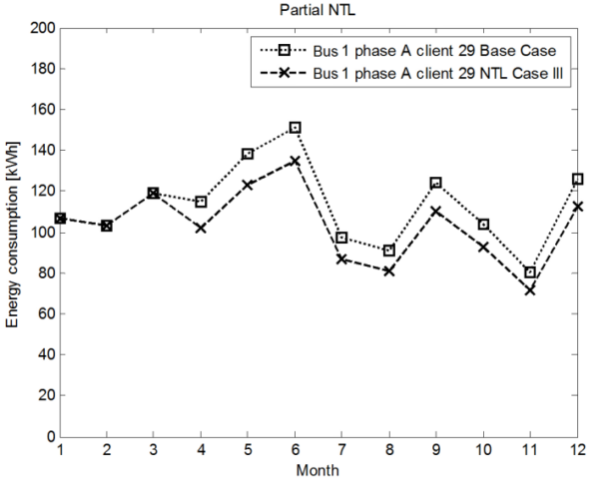
\includegraphics[scale=0.33]{decrease-partial.png}
			\caption{Čiastočné zníženie spotreby elektrickej energie~\cite{Trevizan2015}.}
			\label{fig:decrease-partial}
		\end{center}
	\end{minipage}
  \centering
  \begin{minipage}{0.45\textwidth}
    \begin{center}
      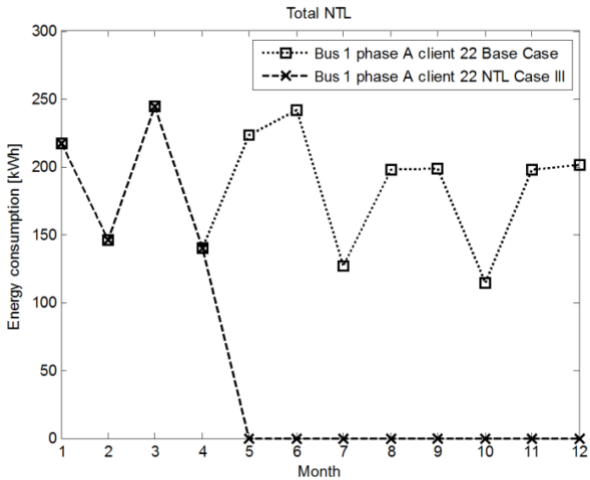
\includegraphics[scale=0.33]{decrease-total.png}
			\caption{Úplné zníženie spotreby elektrickej energie~\cite{Trevizan2015}.}
			\label{fig:decrease-total}
    \end{center}
  \end{minipage}\hfill

\end{figure}

%-------------------------------------------------------------------------------
%   Evaluation metrics
%-------------------------------------------------------------------------------

% TODO add confusion matrix table
\subsection{Vyhodnocovacie metriky}
Za predpokladu, že získané dáta budú obsahovať aj označené inštancie, prípadne
budú označené dodatočne na základe výpočtov, môžeme na vyhodnotenie úspešnosti
použiť aj CONFUSION MATRIX. V~takom prípade budeme musieť predpovedať triedu
jednotlivých inštancií, a~teda či sa jedná o~normálneho alebo anomálneho
odberateľa. Jednoduchý klasifikátor označí prvých \textit{n} odberateľov,
ktorých miera pravdepodobnosti výskytu čierneho odberu je najvyššia, za
anomálnych. Pri použití CONFUSION MATRIX potom riadky predstavujú predpovedanú
triedu a~stĺpce skutočnú. Vznikajú tak 4~kategórie, ktoré sú označované ako
\textit{TRUE POSITIVE} (správne označení podozriví odberatelia),
\textit{FALSE POSITIVE} (nesprávne označení podozriví odberatelia),
\textit{TRUE NEGATIVE} (nesprávne označený normálny odberatelia)
a~\textit{FALSE NEGATIVE} (správne označený normálny odberatelia). Kvalitu
klasifikácie potom môžeme zmerať pomocou presnosti a citlivosti. Presnosť
vypočítame vzorcom~\ref{eq:precision}, kedy ide o~pomer správne označených
anomálií a~celkový počet označených anomálií. Tým vypočítame percento
odberateľov, ktorých sme správne klasifikovali ako podozrivých.
\begin{equation}
	\label{eq:precision}
  \text{Presnosť} = \frac{TP}{TP + FP}
\end{equation}
Citlivosť označuje pomer správne označených anomálií a~celkový počet skutočných
anomálií. Vyjadríme ju pomocou vzorca~\ref{eq:recall}.
\begin{equation}
	\label{eq:recall}
  \text{Citlivosť} = \frac{TP}{TP + FN}
\end{equation}
Aby sa predišlo situácií, kedy sa v~dátach nachádza iba malý počet anomálnych
odberateľov a~pre model by tak bolo výhodnejšie označovať iba tých, s~ktorými si
je takmer istý, je dôležité brať do úvahy aj túto metriku. Obe metriky sú
vyjadrené v~percentách~\cite{Trevizan2015}.

Ďalšou používanou metrikou je aj tzv. F-skóre, ktoré obsahuje informácie oboch
predchádzajúcich metrík. Keďže ide o~súčet metrík, tiež je vyjadrené
v~percentách. Cieľom práce je maximalizovať túto metriku. F-skóre vyjadríme
pomocou vzorca~\ref{eq:f-score}, kde $P$~predstavuje presnosť a~$C$ predstavuje
citlivosť~\cite{Trevizan2015}.
\begin{equation}
	\label{eq:f-score}
  F = 2 \cdot \left( P^{-1} + C^{-1} \right)^{-1}
\end{equation}

%-------------------------------------------------------------------------------
%   Related work
%-------------------------------------------------------------------------------

\subsection{Súvisiace práce v doméne energetiky}
V~\cite{Hautamaki2008} bola pri zhlukovaní použitá aj kombinácia viacerých
metód, konkrétne k-means, metóda náhodnej výmeny a~aglomeratívne zhlukovanie.
Ako už bolo spomenuté v~\ref{c-analysis-techniques}, úlohou algoritmu k-means
namapovať existujúce inštancie do \textit{k} zhlukov. Aj keď metóda náhodnej
výmeny je obmedzená na zhlukovacie problémy v~Euklidovskom priestore, bola
použitá aj pri zhlukovaní časových radov a~zabraňuje zaseknutiu zhluku
v~lokálnom minime. V~princípe je náhodne vybraný zhluk, ktorý bude vymazaná a~za
centroid bude vybraný jeden časový rad z~neho. Ak takéto riešenie je lepšie ako
bez rozpustenia zhluku je nahradené pôvodným. Ako bolo spomenuté
v~\ref{c:hierarchical-clustering} cieľom aglomeratívneho zhlukovania je všetky
časové rady označiť ako zhluky a~následne ich iteratívne zhlukovať. V~momente,
keď je vytvorených \textit{k} zhlukov, je vypočítaný centroid zhluku a~určená
hierarchia zhlukov.\\

V~práci~\cite{Cody2015} boli pri určovaní podozrivých aktivít odberateľov
úspešne aplikované rozhodovacie stromy. Po vytvorení trénovacej a~testovacej
množiny boli vygenerované rozhodovacie pravidlá reprezentujúce model normálnej
spotreby elektrickej energie. Po predikcii boli porovnané predikované
a~testovacie dáta pomocou štatistickej metódy RMSE. Výsledkom experimentov je
dostatočne presná predikcia spotreby energie vypočítaná iba na základe atribútov
extrahovaných z~časovej známky. Prekročením stanovej hranice boli inštancie
považované za anomálne.  Počas experimentov boli použité M5P rozhodovacie učiace
stromy.\\

Predmetom článku~\cite{Tagaris2002} bolo navrhnúť novú vlnovú techniku na
reprezentovanie viacerých vlastností meraných dát. Tiež vytvorili nový model,
ktorý v~sebe zahŕňa viacero modelov, čím je pridávanie ďalších komponentov do
detekčného systému jednoduché. Navrhovaná metóda je citlivá na lokálne zmeny vo
vzore dát. Taktiež dosiahli s~relatívne malým množstvom meraní presnosť až 78\%
na trénovacej množine a~70\% na testovacej množine. Metóda je citlivá na zmeny
amplitúd a~frekvencií v~dátach z~meračov. Nevýhodou je, že model nie je citlivý
na nevýrazne zmeny a~trendy v~dátach.\\

%-------------------------------------------------------------------------------
%   Chapter 3 - Requirements specification
%-------------------------------------------------------------------------------

\newpage
\section{Špecifikácia požiadaviek}
\section{Rozpracovanie problému}
Pomocou metód strojového učenia a~dátovej analytiky sa zameriame na identifikáciu
anomálií v~oblasti distribučných spoločností. Na základe dát, ktoré máme
k~dispozícií zvolíme vhodnú metódu detekcie anomálií. Keďže dáta sú z~domény
distribúcie elektrickej energie, ich označenie by bolo finančne aj časovo
náročné. Rovnako aj spätná väzba pri identifikácií anomálií je časovo náročná
a~jej spracovanie môže trvať niekoľko týždňov až mesiacov.

Zameriavať sa budeme najmä na identifikáciu anomálií v~časových radoch, čo spadá
pod skupinové a~kontextové typy anomálií. Úlohou bude taktiež identifikovať
výhody a~nevýhody uplatnenia jednotlivých prístupov k~identifikácií. Zároveň
vzniká potreba nájsť najvhodnejšie techniky detekcií anomálií pre dáta zbierané
z~distribučných sietí pomocou inteligentných meračov. Najmä z~dôvodu, že každá
doména, v~ktorej je potrebné identifikovať anomálie sa vyznačuje špecifickými
potrebami na použitý model.


%-------------------------------------------------------------------------------
%   Chapter 8 - Bibliography
%-------------------------------------------------------------------------------

\newpage
\bibliographystyle{iso-690/slovakiso}
\bibliography{bibliography}

\end{document}

% \subsubsection{Nájdenie anomálií}
% \paragraph{Klasifikácia}
% \paragraph{Identifikácia najbližším susedom}
% \paragraph{Identifikácia zhlukovaním}
% \paragraph{Grafová analýza}
% \paragraph{Štatistické metódy}
% \paragraph{Hybridné prístupy}
% \paragraph{Spektrálna analýza}
